\section{Resultados Obtidos}
\label{sec:resultados}

\subsection{Caracterização dos dados}
\label{subsec:caracterizacao_resultados}

A Tabela~\ref{tab:caracterizacao_sensores} apresenta a disponibilidade
e as estatísticas das temperaturas agregadas no período consultado.
As estatísticas foram calculadas com as janelas válidas de cada sensor,
antes da seleção das linhas completas. A cobertura variou de 97,39\%
a 97,85\%. A utilização conjunta dos nove sensores reteve 12.892
das 13.248 janelas, correspondendo a 97,31\% da grade temporal.

\begin{table}[htbp]
    \centering
    \caption{Disponibilidade e estatísticas das médias de cinco minutos.}
    \label{tab:caracterizacao_sensores}
    \small
    \begin{tabular}{rrrrrr}
\toprule
Sensor & Janelas válidas & Ausentes & Cobertura (\%) & Média (°C) & Desvio (°C) \\
\midrule
1 & 12944 & 304 & 97,71 & 21,994 & 1,185 \\
48 & 12902 & 346 & 97,39 & 22,113 & 0,993 \\
887 & 12931 & 317 & 97,61 & 22,617 & 1,154 \\
891 & 12954 & 294 & 97,78 & 19,847 & 0,805 \\
86782 & 12963 & 285 & 97,85 & 22,002 & 1,187 \\
86789 & 12918 & 330 & 97,51 & 21,551 & 1,172 \\
86790 & 12925 & 323 & 97,56 & 24,019 & 1,155 \\
86791 & 12941 & 307 & 97,68 & 23,275 & 1,168 \\
86793 & 12960 & 288 & 97,83 & 22,494 & 1,277 \\
\bottomrule
\end{tabular}

    \fautor
\end{table}

As médias temporais diferem entre dispositivos: o sensor 891
apresentou 19,847~°C, enquanto o sensor 86790 apresentou 24,019~°C.
Essas diferenças mostram que a média indiscriminada dos demais
sensores pode não representar o nível térmico de todos os alvos.
Entretanto, as estatísticas não permitem atribuir tais diferenças
a causas específicas, como posição, climatização ou calibração.

\subsection{Comparação entre métodos}
\label{subsec:comparacao_metodos}

A Tabela~\ref{tab:comparacao_modelos} resume o desempenho no teste.
Os métodos supervisionados apresentaram menores erros médios entre
alvos que a média aritmética. A Random Forest obteve MAE médio de
0,254~°C, e a regressão linear, 0,257~°C. A diferença de MAE foi
aproximadamente 0,0024~°C. Por outro lado, a regressão linear apresentou
menor média dos RMSE: 0,325~°C, contra 0,332~°C da Random Forest.
Não houve, portanto, predominância do mesmo método nas duas métricas,
e não foi realizado teste de significância estatística dessa diferença.

\begin{table}[htbp]
    \centering
    \caption{Médias das métricas entre os nove sensores-alvo no teste.}
    \label{tab:comparacao_modelos}
    \begin{tabular}{lrrr}
\toprule
Método & MAE (°C) & RMSE (°C) & $R^2$ \\
\midrule
Média aritmética & 0,927 & 0,991 & -2,362 \\
Random Forest & 0,254 & 0,332 & 0,852 \\
Regressão linear & 0,257 & 0,325 & 0,850 \\
\bottomrule
\end{tabular}

    \fautor
\end{table}

O $R^2$ médio negativo da média aritmética não implica desempenho
negativo em todos os alvos. Sua agregação é fortemente influenciada
pelo sensor 891, para o qual esse método obteve $R^2=-23,519$, e
pelo sensor 86790, com $R^2=-2,497$. Um $R^2$ negativo indica erro
quadrático superior ao da referência constante igual à média do
próprio alvo no teste; essa referência serve à definição da métrica
e não foi utilizada como entrada dos modelos.

\subsection{Diferenças entre sensores-alvo}
\label{subsec:resultados_por_alvo}

A Tabela~\ref{tab:mae_alvos} e a Figura~\ref{fig:mae_alvos}
mostram que a comparação global não se aplica uniformemente aos
dispositivos. A regressão linear apresentou o menor MAE em quatro
alvos (48, 86789, 86790 e 86793), a Random Forest em três (887,
891 e 86791) e a média aritmética em dois (1 e 86782).

\begin{table}[htbp]
    \centering
    \caption{MAE por sensor-alvo e método, em graus Celsius.}
    \label{tab:mae_alvos}
    \begin{tabular}{rrrr}
\toprule
Sensor-alvo & Média aritmética & Regressão linear & Random Forest \\
\midrule
1 & 0,145 & 0,240 & 0,202 \\
48 & 0,253 & 0,155 & 0,167 \\
887 & 0,462 & 0,276 & 0,264 \\
891 & 2,989 & 0,387 & 0,374 \\
86782 & 0,198 & 0,399 & 0,342 \\
86789 & 0,705 & 0,090 & 0,110 \\
86790 & 2,014 & 0,145 & 0,176 \\
86791 & 1,041 & 0,379 & 0,352 \\
86793 & 0,540 & 0,240 & 0,303 \\
\bottomrule
\end{tabular}

    \fautor
\end{table}

\begin{figure}[htbp]
    \centering
    \caption{Comparação do MAE por sensor-alvo no conjunto de teste.}
    \label{fig:mae_alvos}
    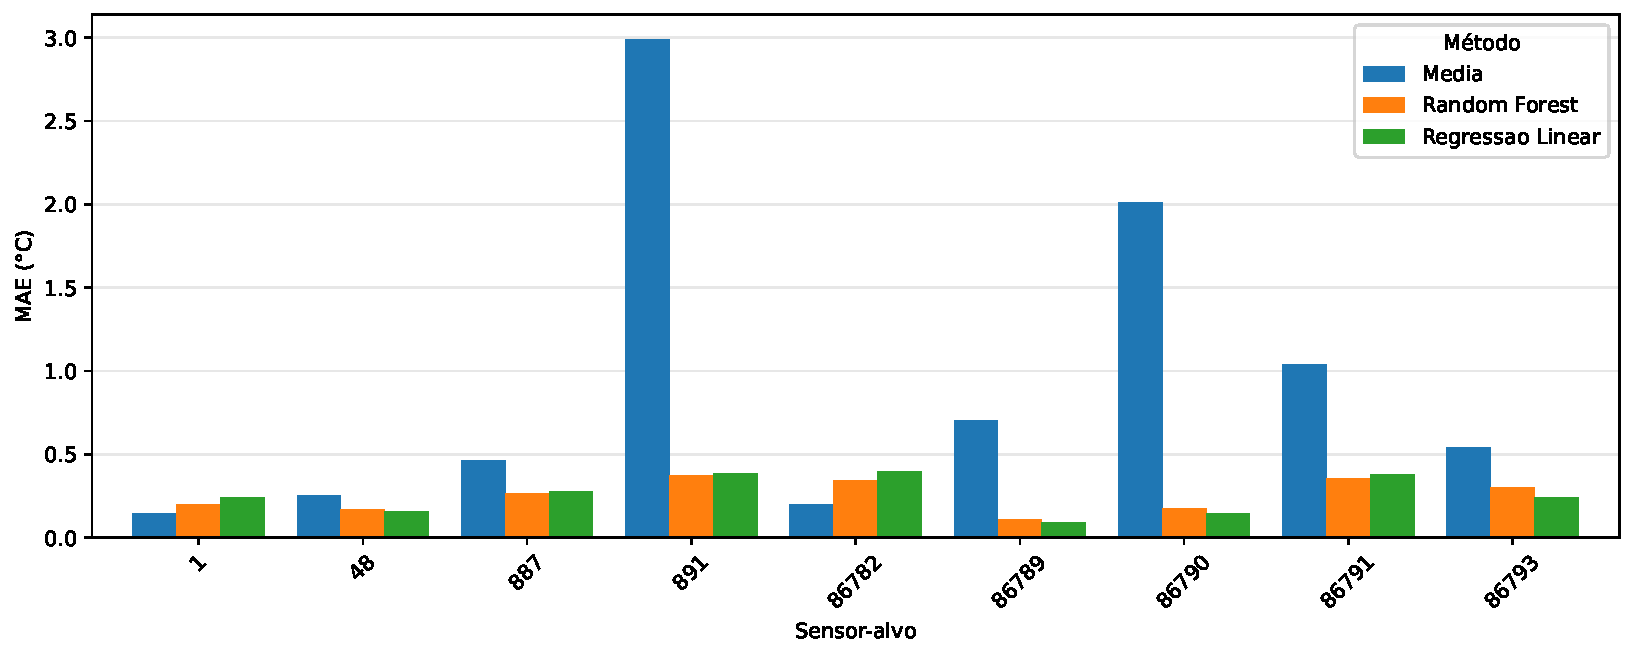
\includegraphics[width=\linewidth]{mae_por_sensor.pdf}
    \fautor
\end{figure}

O sensor 86789 apresentou o menor MAE supervisionado: 0,090~°C
com regressão linear, acompanhado de $R^2=0,985$. Já o sensor 891
apresentou MAE de 0,387~°C com regressão linear e 0,374~°C com
Random Forest, cujos $R^2$ foram, respectivamente, 0,442 e 0,448.
Assim, erros absolutos inferiores a meio grau nesse alvo coexistiram
com uma parcela relevante de variação não explicada pelos modelos.

Nos sensores 1 e 86782, a média aritmética obteve MAE de 0,145~°C
e 0,198~°C, respectivamente, abaixo dos dois modelos supervisionados.
Esse resultado evidencia a importância de manter uma referência
simples e avaliar cada alvo. O ajuste no treinamento não garante
menor erro no período posterior para todos os dispositivos.

A Figura~\ref{fig:reconstrucao_891} apresenta o sensor 891 como
exemplo das dificuldades de reconstrução, escolhido por seu maior
MAE entre os alvos na Random Forest. Os gráficos dos demais alvos
foram igualmente exportados. Nesse exemplo, a média aritmética
permanece acima da temperatura observada, enquanto as estimativas
supervisionadas acompanham melhor seu nível, mas ainda apresentam
resíduos positivos em parte do teste. A figura permite visualizar
esse comportamento, sem estabelecer sua causa física.

\begin{figure}[htbp]
    \centering
    \caption{Temperaturas observadas, estimativas e resíduos do sensor 891.}
    \label{fig:reconstrucao_891}
    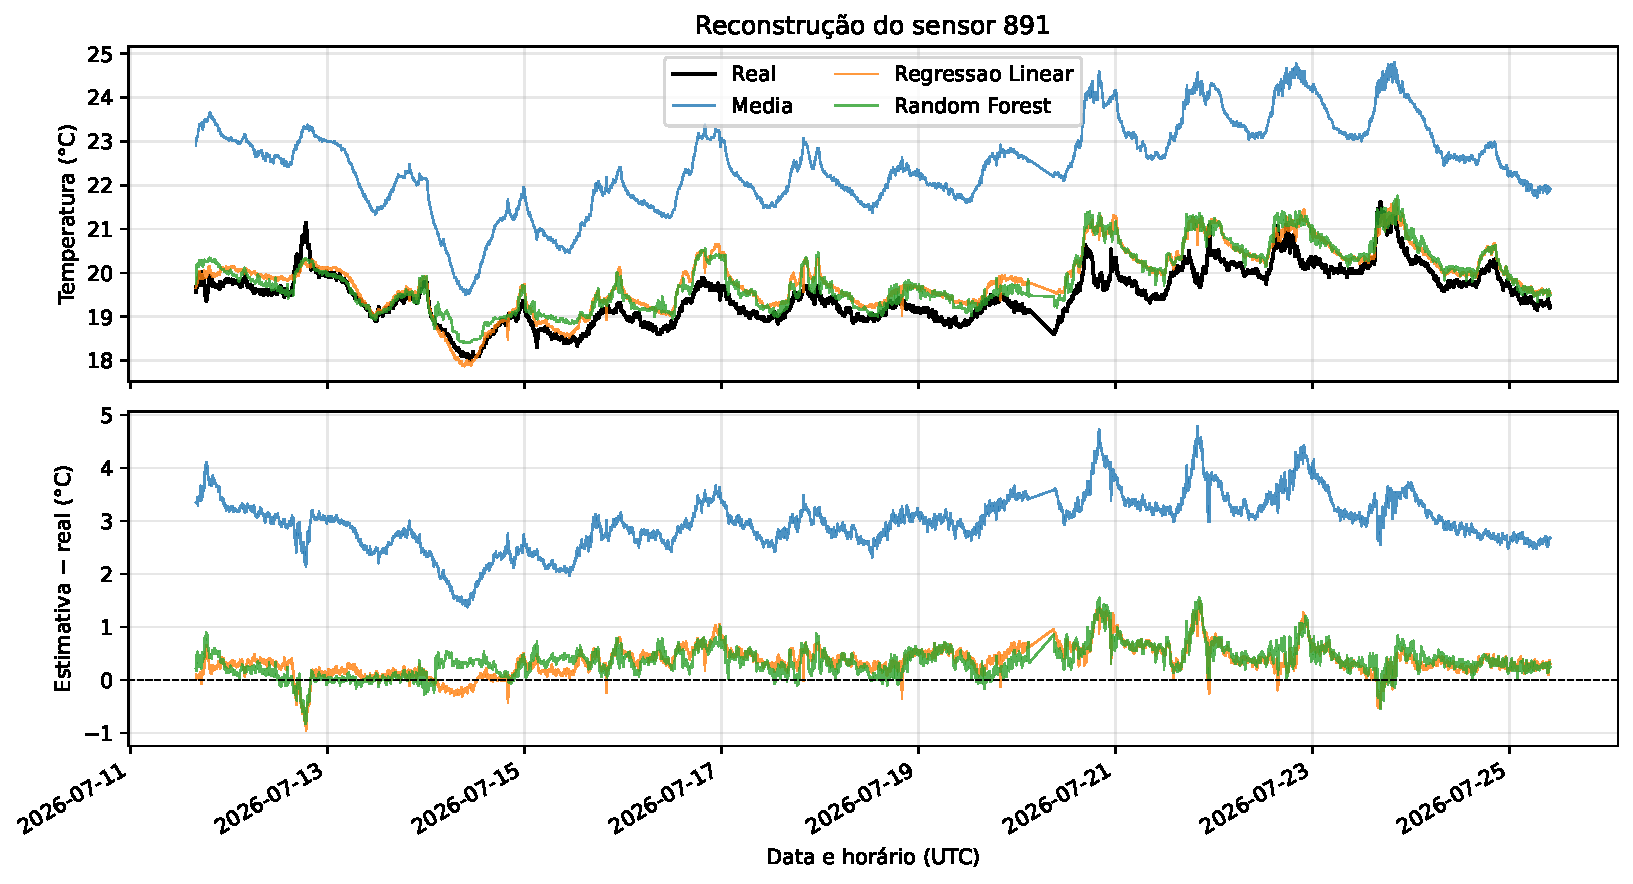
\includegraphics[width=\linewidth]{reconstrucao_sensor_891.pdf}
    \fautor
\end{figure}

\subsection{Influência da quantidade de entradas}
\label{subsec:resultados_quantidade}

A Tabela~\ref{tab:quantidade_sensores} apresenta os resultados da
regressão linear com seleção por correlação no treinamento.
O MAE médio diminuiu de 0,296~°C com uma entrada para 0,238~°C
com quatro. Com seis e oito entradas, os valores aumentaram para
0,257~°C, aproximadamente. A média dos RMSE também atingiu seu
menor valor entre as configurações avaliadas com quatro entradas,
igual a 0,302~°C.

\begin{table}[htbp]
    \centering
    \caption{Médias das métricas da regressão linear por quantidade de entradas.}
    \label{tab:quantidade_sensores}
    \begin{tabular}{rrrr}
\toprule
$k$ & MAE (°C) & RMSE (°C) & $R^2$ \\
\midrule
1 & 0,296 & 0,370 & 0,816 \\
2 & 0,255 & 0,322 & 0,855 \\
3 & 0,245 & 0,311 & 0,875 \\
4 & 0,238 & 0,302 & 0,880 \\
6 & 0,257 & 0,325 & 0,864 \\
8 & 0,257 & 0,325 & 0,850 \\
\bottomrule
\end{tabular}

    \fautor
\end{table}

A Figura~\ref{fig:quantidade_sensores} evidencia que o comportamento
varia conforme o alvo. Para o sensor 86782, por exemplo, o erro
cresce ao aumentar o número de entradas no ordenamento adotado,
enquanto outros sensores se beneficiam da inclusão de variáveis.
Portanto, o menor erro médio com quatro entradas não implica que
esse número seja preferível para todos os alvos.

\begin{figure}[htbp]
    \centering
    \caption{Erros por alvo e médias em função da quantidade de entradas.}
    \label{fig:quantidade_sensores}
    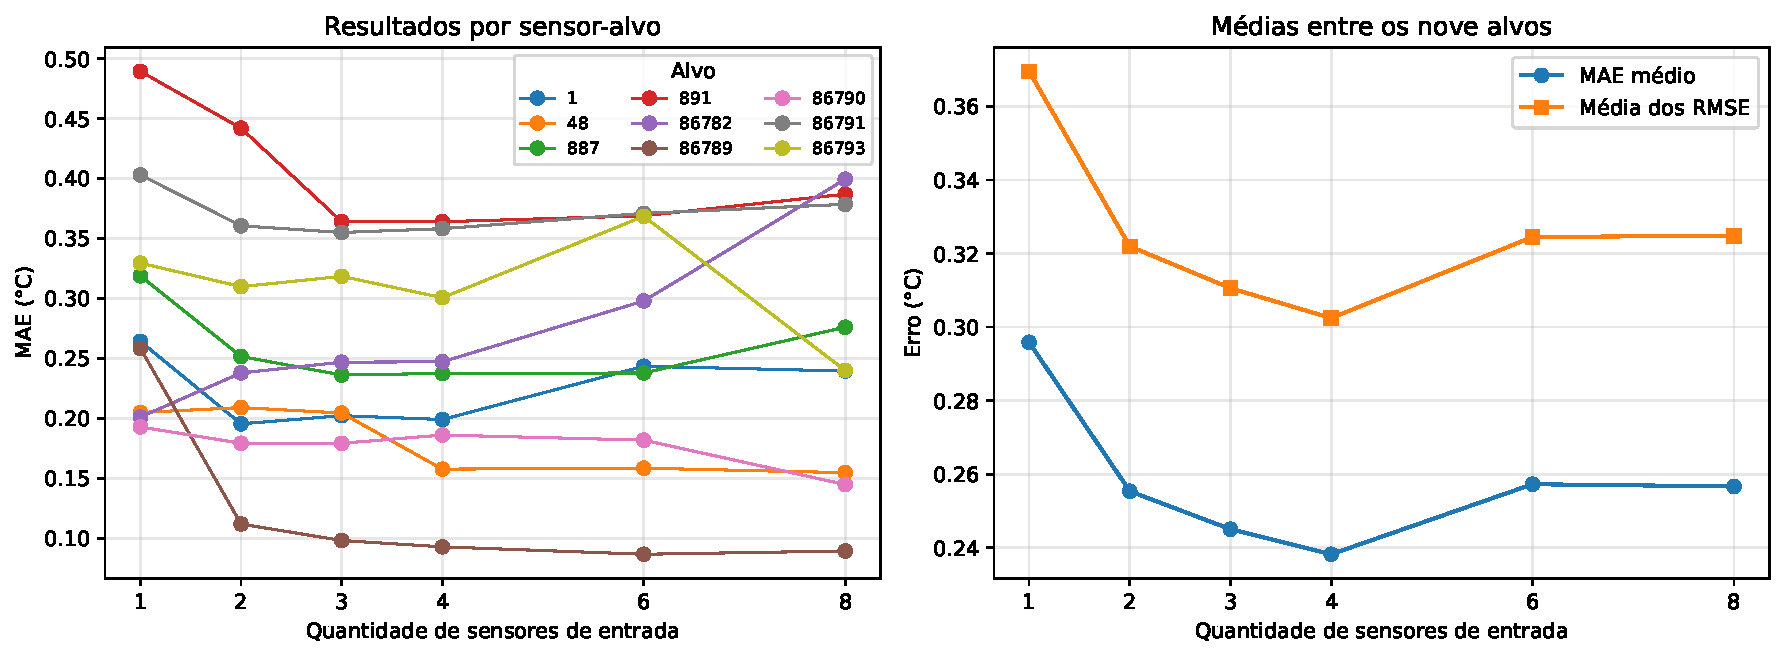
\includegraphics[width=\linewidth]{erro_quantidade_sensores.pdf}
    \fautor
\end{figure}

Esses resultados indicam que, neste período e com essa regra de
seleção, utilizar todos os sensores disponíveis não produziu o
menor erro médio. Entretanto, não demonstram que a seleção por
correlação supera outros critérios, pois não houve comparação
com subconjuntos aleatórios ou selecionados por distância nesse conjunto
de nove sensores. A comparação espacial complementar utiliza um recorte
comum de seis sensores e é apresentada na
Seção~\ref{subsec:resultados_espaciais}.
Também não estabelecem uma quantidade ótima geral: quatro foi
o menor erro observado entre os valores de $k$ examinados nesse
teste, sem uma avaliação independente posterior à escolha.

\subsection{Disponibilidade dos dados nas fontes consultadas}
\label{subsec:disponibilidade_fontes}

As extrações locais evidenciam diferenças no conjunto de dispositivos
consultados em cada fonte. O experimento principal contém nove sensores
do ambiente 1006 no QuestDB. A coleta pela API Smartlab contém 14
sensores com coordenadas: seis do ambiente 1006, seis do cluster e
dois cadastrados na reunião. Seis identificadores estão presentes
em ambas as extrações. Os sensores 1, 86782 e 86789 fazem parte da
extração principal do QuestDB, mas não da coleta local de 14 sensores
da Smartlab. Essa ausência decorre do inventário consultado e não
demonstra indisponibilidade desses dispositivos em toda a API.

Na consulta exploratória ao QuestDB preservada no notebook original,
a busca pelos seis identificadores do cluster retornou um conjunto
vazio, enquanto a API permitiu obter registros desses mesmos dispositivos.
Esse achado documenta o resultado das consultas realizadas, sem
estabelecer que as duas fontes tenham cobertura histórica equivalente
ou que o estado dos servidores permaneça o mesmo.

As respostas locais da API contêm timestamps sem indicação de fuso
e intervalos observados inferiores aos cinco minutos solicitados na
configuração exploratória. Assim, a contagem dessas linhas não pode
ser comparada diretamente à quantidade de janelas válidas do QuestDB.
A equiparação exige verificar a semântica temporal e a agregação antes
de combinar os dados. Por esse motivo, o mapa e a avaliação espacial
utilizam somente temperaturas do QuestDB, embora mostrem as posições
cadastradas dos demais dispositivos.

\subsection{Coordenadas e comparação da seleção espacial}
\label{subsec:resultados_espaciais}

A Tabela~\ref{tab:coordenadas} relaciona as posições confirmadas dos
seis sensores usados na análise complementar. As médias dessa tabela
utilizam somente as janelas completas comuns aos nove sensores do
experimento principal, diferentemente das estatísticas por sensor
da Tabela~\ref{tab:caracterizacao_sensores}.

\begin{table}[htbp]
    \centering
    \caption{Coordenadas relativas e médias nas 12.892 janelas comuns.}
    \label{tab:coordenadas}
    \begin{tabular}{rrrr}
\toprule
Sensor & X relativo & Y relativo & Média (°C) \\
\midrule
48 & 8,0 & 5,6 & 22,114 \\
887 & 0,0 & 0,0 & 22,618 \\
891 & 0,0 & 4,9 & 19,850 \\
86790 & 3,0 & 1,4 & 24,019 \\
86791 & 5,0 & 1,4 & 23,276 \\
86793 & 8,0 & 0,0 & 22,497 \\
\bottomrule
\end{tabular}

    \fautor
\end{table}

A Tabela~\ref{tab:selecao_espacial} e a Figura~\ref{fig:selecao_espacial}
apresentam a comparação entre seleção por correlação e por proximidade.
Para uma a quatro entradas, a correlação apresentou menor MAE médio
entre os seis alvos. Com uma entrada, os MAE médios foram 0,315~°C
para correlação e 0,390~°C para proximidade; com quatro, foram
0,276~°C e 0,295~°C, respectivamente. A média dos RMSE também foi
menor para a seleção por correlação nesses quatro valores de $k$.

\begin{table}[htbp]
    \centering
    \caption{Seleção por correlação e proximidade: médias entre seis alvos (°C).}
    \label{tab:selecao_espacial}
    \begin{tabular}{rrrrr}
\toprule
$k$ & MAE corr. & RMSE corr. & MAE prox. & RMSE prox. \\
\midrule
1 & 0,315 & 0,417 & 0,390 & 0,488 \\
2 & 0,298 & 0,379 & 0,374 & 0,458 \\
3 & 0,285 & 0,365 & 0,367 & 0,459 \\
4 & 0,276 & 0,353 & 0,295 & 0,374 \\
5 & 0,266 & 0,346 & 0,266 & 0,346 \\
\bottomrule
\end{tabular}

    \fonte{Autor desta monografia. Corr.: correlação; prox.: proximidade.}
\end{table}

\begin{figure}[htbp]
    \centering
    \caption{Desempenho da regressão linear com duas regras de seleção.}
    \label{fig:selecao_espacial}
    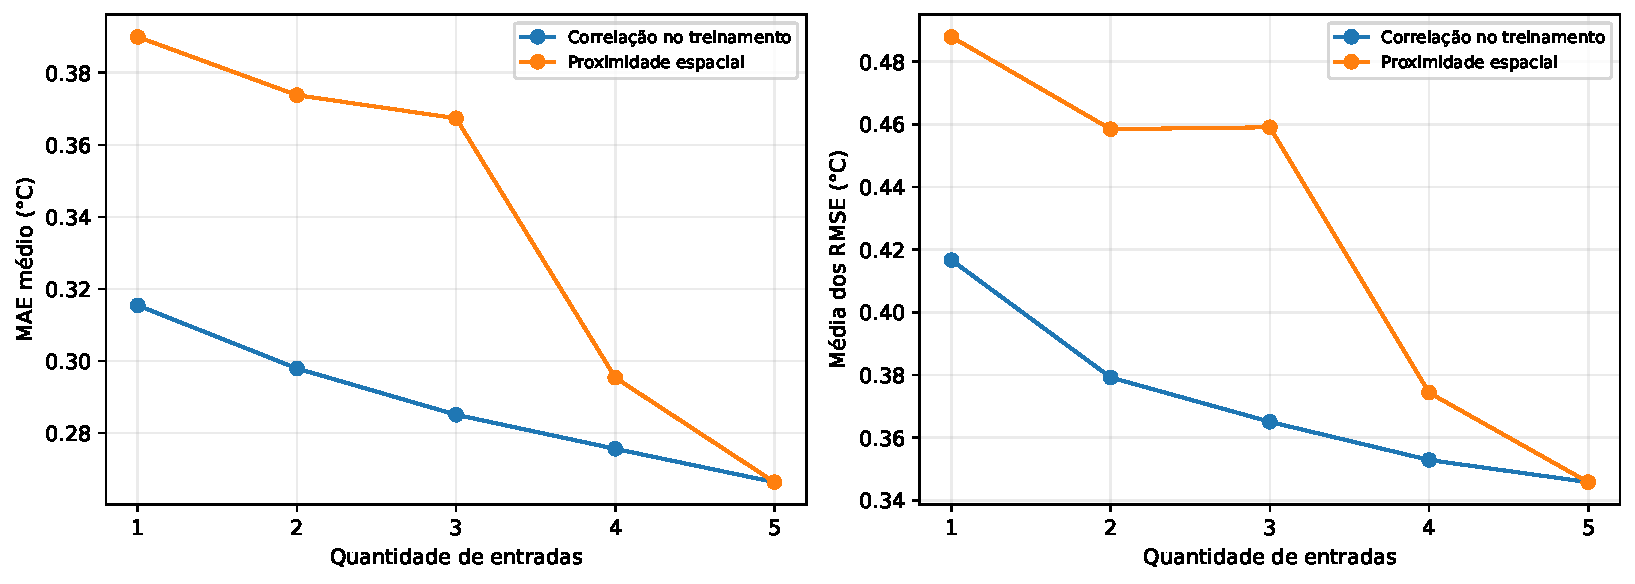
\includegraphics[width=\linewidth]{comparacao_selecao_espacial.pdf}
    \fautor
\end{figure}

Com cinco entradas, as duas regras utilizaram o mesmo conjunto de
sensores e produziram MAE médio de 0,266~°C e média dos RMSE de
0,346~°C. A concordância confirma a consistência dessa comparação.
Os resultados sugerem que a distância, isoladamente, não capturou
as relações úteis à regressão tão bem quanto a correlação histórica
nessa configuração. Não foi realizado teste de significância ou
validação em períodos adicionais para generalizar essa diferença.

A seleção espacial é uma análise com seis candidatos e seis alvos.
Seus erros médios não devem ser comparados diretamente aos da
Tabela~\ref{tab:quantidade_sensores}, que considera nove sensores.
Em particular, o menor erro com cinco entradas neste recorte não
contradiz o resultado com quatro entradas no conjunto anterior.
A divisória também não foi avaliada como variável explicativa ou
como efeito causal: ela é uma condição física documentada, e os
sensores do cluster foram excluídos dos candidatos de ambas as regras.

\subsection{Distribuição espacial das temperaturas médias}
\label{subsec:mapa_termico}

A Figura~\ref{fig:mapa_termico} apresenta os valores médios medidos
nos seis pontos e a interpolação ilustrativa entre eles. O sensor
891, localizado abaixo da divisória, apresentou média de 19,850~°C,
enquanto o sensor 86790 apresentou 24,019~°C. A figura permite
situar espacialmente essa diferença, sem atribuí-la à divisória,
aos equipamentos ou à climatização.

\begin{figure}[htbp]
    \centering
    \caption{Temperaturas médias observadas e interpolação IDW ilustrativa.}
    \label{fig:mapa_termico}
    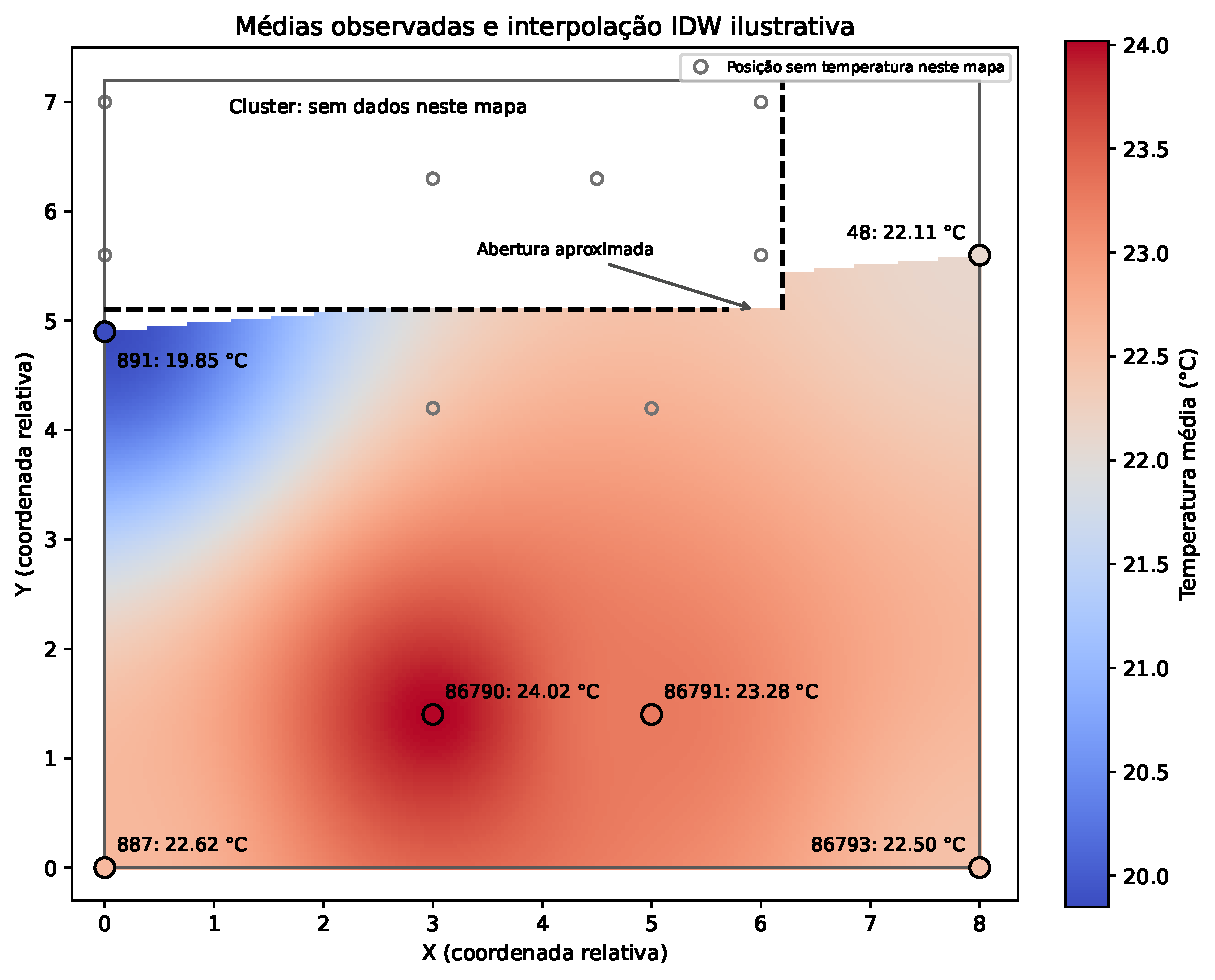
\includegraphics[width=0.95\linewidth]{mapa_termico_1006_painel.pdf}
    \fonte{Autor desta monografia. Geometria aproximada a partir da planta;
    pontos coloridos: médias observadas; fundo: interpolação das médias.
    Regiões sem preenchimento não foram estimadas.}
\end{figure}

A área do cluster permanece sem preenchimento, evitando apresentar
uma continuidade interpolada através da divisória. As paredes
tracejadas e a abertura aproximada indicam a limitação geométrica
da representação. A IDW suaviza as médias entre os pontos observados,
mas não fornece evidência de que as temperaturas nas posições sem
sensores correspondam aos valores coloridos. O mapa complementa a
caracterização dos dados; a validação quantitativa continua restrita
aos sensores físicos usados como alvos.

\subsection{Caracterização da umidade e efeito do enriquecimento}
\label{subsec:resultados_umidade}

A Tabela~\ref{tab:umidade_sensores} apresenta a disponibilidade da
umidade e as estatísticas das médias de cinco minutos, antes de
restringir as amostras à comparação pareada. A cobertura variou de
97,52\% a 97,85\% da grade. As umidades médias variaram de 53,98\%
no sensor 86790 a 59,80\% no sensor 891. O desvio é expresso em
pontos percentuais (p.p.), para distinguir a variação da UR de uma
variação percentual relativa à média.

\begin{table}[htbp]
    \centering
    \caption{Disponibilidade e estatísticas da umidade relativa agregada.}
    \label{tab:umidade_sensores}
    \begin{tabular}{rrrrr}
\toprule
Sensor & Janelas & Cobertura (\%) & Média (\%) & Desvio (p.p.) \\
\midrule
1 & 12944 & 97,71 & 56,65 & 8,47 \\
48 & 12919 & 97,52 & 54,52 & 8,06 \\
887 & 12931 & 97,61 & 57,66 & 7,48 \\
891 & 12954 & 97,78 & 59,80 & 7,09 \\
86782 & 12963 & 97,85 & 56,57 & 8,67 \\
86789 & 12938 & 97,66 & 57,14 & 8,25 \\
86790 & 12925 & 97,56 & 53,98 & 7,25 \\
86791 & 12941 & 97,68 & 56,75 & 7,25 \\
86793 & 12960 & 97,83 & 59,16 & 8,19 \\
\bottomrule
\end{tabular}

    \fautor
\end{table}

A Figura~\ref{fig:caracterizacao_umidade} mostra a evolução das
médias horárias, utilizadas apenas para legibilidade, e a proporção
de janelas válidas de cinco minutos. As correlações de Pearson
entre temperatura e umidade do mesmo dispositivo, calculadas no
treinamento, foram negativas nos nove sensores, entre $-0{,}446$
e $-0{,}108$. Esse diagnóstico não demonstra que a umidade forneça
informação preditiva adicional; essa possibilidade foi examinada
na comparação com entradas enriquecidas.

\begin{figure}[htbp]
    \centering
    \caption{Séries de umidade e disponibilidade das janelas no período.}
    \label{fig:caracterizacao_umidade}
    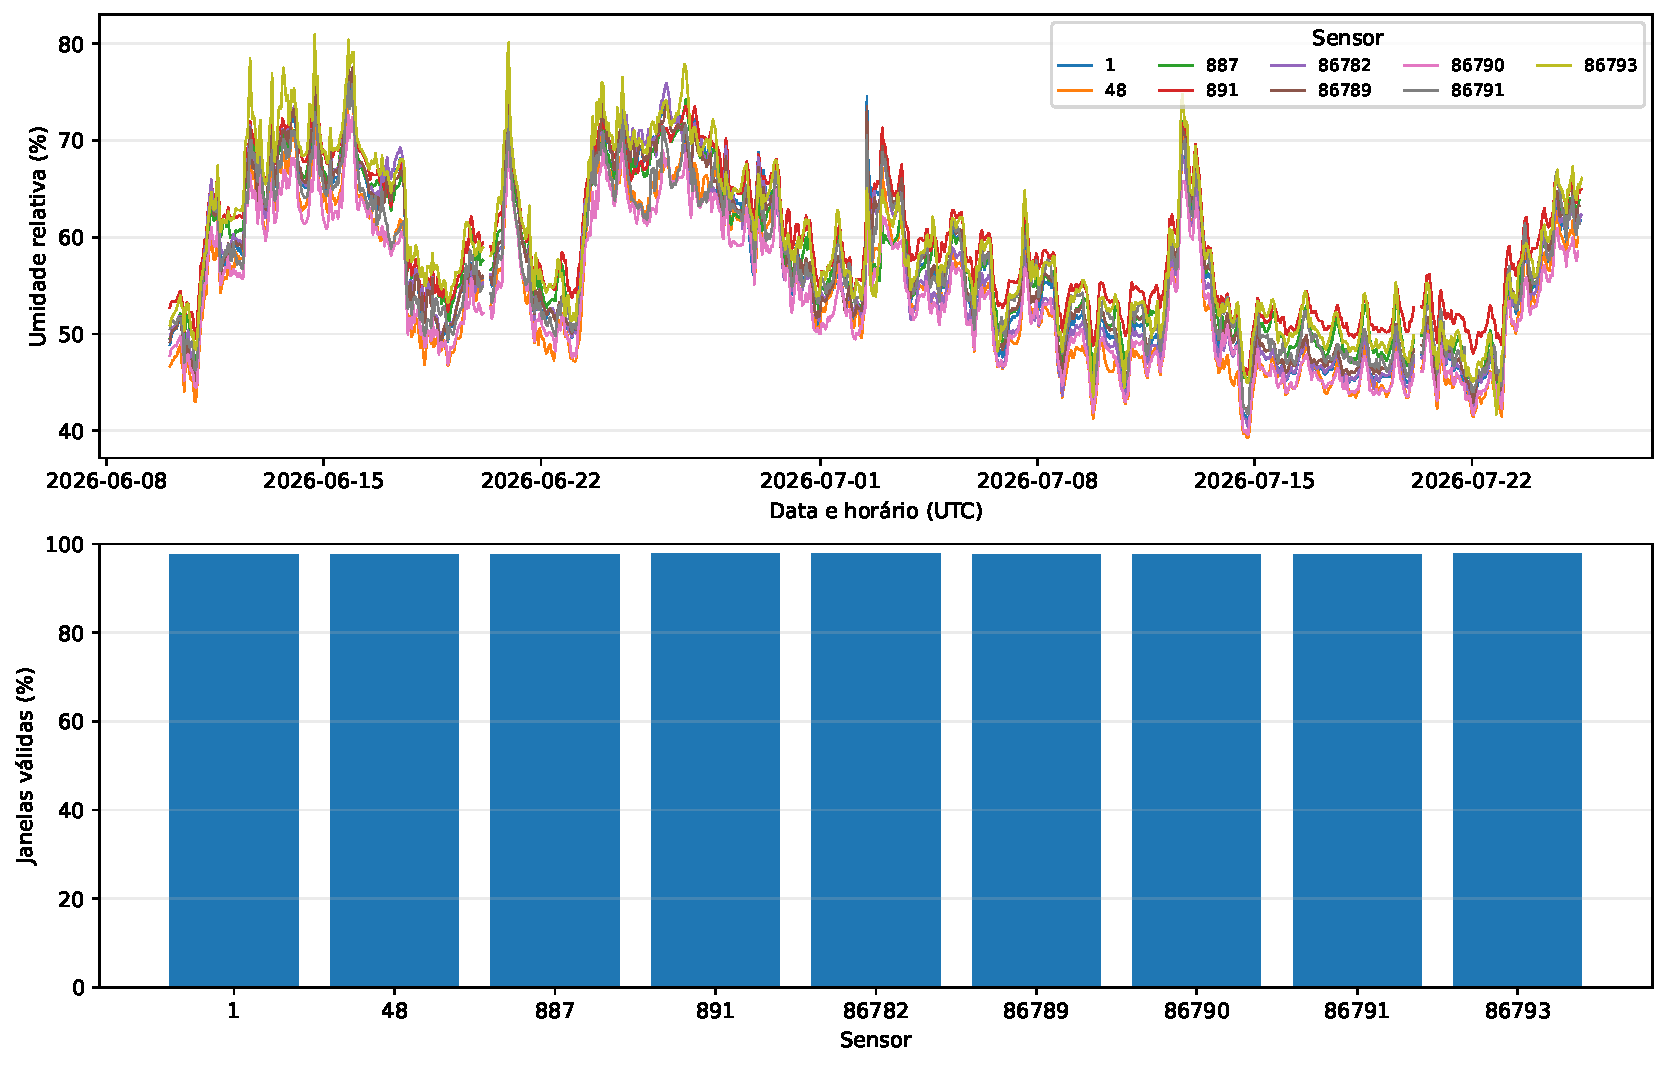
\includegraphics[width=0.95\linewidth]{caracterizacao_umidade.pdf}
    \fautor
\end{figure}

Na Tabela~\ref{tab:enriquecimento_umidade}, o acréscimo de umidade
reduziu o MAE médio da regressão linear de 0,25668~°C para
0,25343~°C, uma diferença de aproximadamente 0,00325~°C.
A média dos RMSE passou de 0,32488~°C para 0,32250~°C.
O ganho agregado foi pequeno e não foi submetido a teste de
significância ou confirmado em períodos independentes.

\begin{table}[htbp]
    \centering
    \caption{Regressão linear com e sem umidade, nas mesmas amostras por alvo.}
    \label{tab:enriquecimento_umidade}
    \begin{tabular}{lrrr}
\toprule
Entradas & MAE (°C) & RMSE (°C) & $R^2$ \\
\midrule
Temperaturas & 0,25668 & 0,32488 & 0,850 \\
Temperaturas e umidades & 0,25343 & 0,32250 & 0,857 \\
\bottomrule
\end{tabular}

    \fautor
\end{table}

A Tabela~\ref{tab:umidade_por_alvo} e a Figura~\ref{fig:efeito_umidade}
mostram que o enriquecimento reduziu o MAE em cinco alvos e aumentou
em quatro. O sensor 891 apresentou redução de 0,38690~°C para
0,33541~°C; já o sensor 86782 passou de 0,39943~°C para
0,45071~°C. Assim, acrescentar uma grandeza ambiental não assegurou
melhora uniforme. A avaliação não permite atribuir o resultado a
uma causa específica, como posição, climatização ou mecanismo físico
entre temperatura e umidade.

\begin{table}[htbp]
    \centering
    \caption{Efeito da umidade no MAE por alvo; diferença negativa indica redução.}
    \label{tab:umidade_por_alvo}
    \begin{tabular}{rrrr}
\toprule
Sensor & Somente T (°C) & T e UR (°C) & $\Delta$ MAE (°C) \\
\midrule
1 & 0,240 & 0,228 & -0,011 \\
48 & 0,155 & 0,169 & 0,014 \\
887 & 0,276 & 0,241 & -0,035 \\
891 & 0,387 & 0,335 & -0,051 \\
86782 & 0,399 & 0,451 & 0,051 \\
86789 & 0,090 & 0,119 & 0,029 \\
86790 & 0,145 & 0,148 & 0,003 \\
86791 & 0,379 & 0,361 & -0,018 \\
86793 & 0,240 & 0,229 & -0,011 \\
\bottomrule
\end{tabular}

    \fautor
\end{table}

\begin{figure}[htbp]
    \centering
    \caption{MAE da regressão linear com e sem umidade dos sensores de entrada.}
    \label{fig:efeito_umidade}
    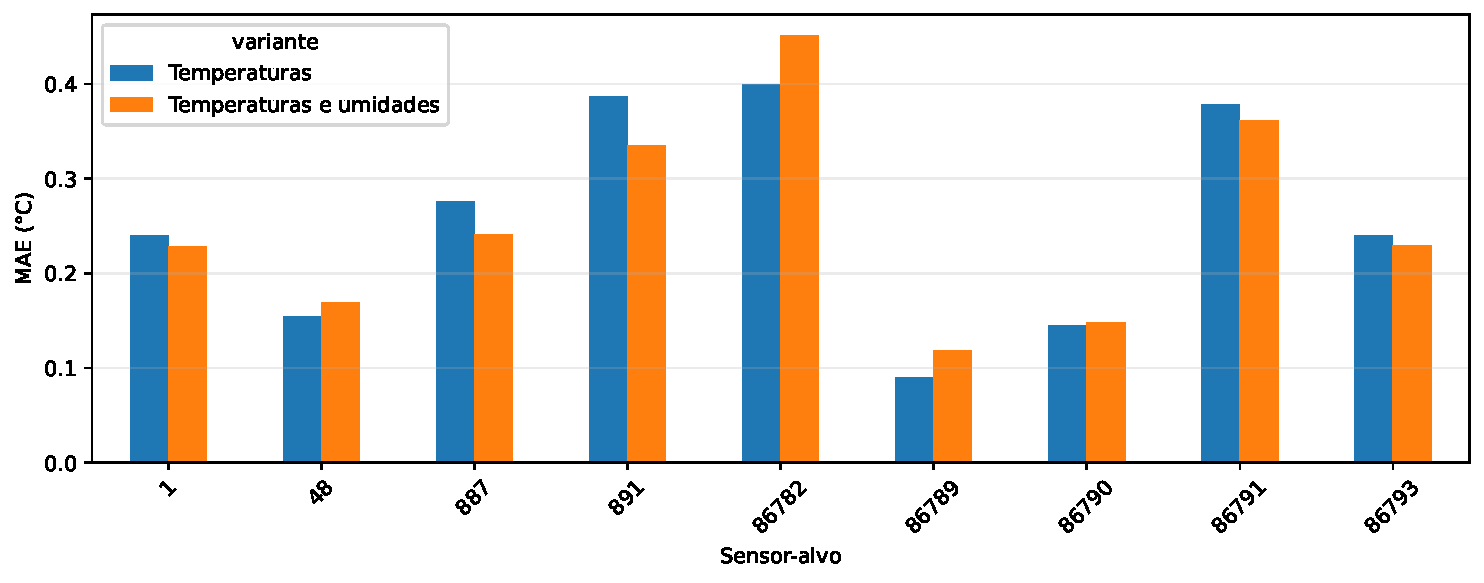
\includegraphics[width=\linewidth]{efeito_umidade.pdf}
    \fautor
\end{figure}

As duas variantes compartilham amostras em cada alvo, mas há duas
linhas de teste a menos para oito alvos em relação ao experimento
principal. Por isso, a referência dessa comparação é a regressão
reajustada com somente temperaturas, e não uma comparação direta
com a Random Forest ou com as médias da
Tabela~\ref{tab:comparacao_modelos}. A análise mantém temperatura
como resposta; a reconstrução da própria umidade não foi avaliada.

\subsection{Disponibilidade e interpretação dos registros de energia}
\label{subsec:resultados_energia}

A consulta à tabela de energia retornou registros apenas do sensor 23
no período selecionado: 8.193 linhas, entre 10/06/2026 às
01h43min35s e 11/06/2026 às 22h31min36s, em UTC. O sensor 2,
identificado na exploração histórica, não retornou dados nesse
recorte. A agregação produziu 539 janelas válidas, correspondentes
a 4,07\% das 13.248 previstas. Portanto, essa fonte não oferece
cobertura comparável à de temperatura e umidade ao longo das seis
semanas analisadas.

Os valores brutos do campo variaram de 0 a 9,13. As médias de cinco
minutos variaram de 0 a 6,865, na escala registrada no banco.
Como a unidade e a transformação do firmware não foram confirmadas,
esses valores não são interpretados como kWh, W ou A. A
Figura~\ref{fig:energia_exploratoria} apresenta apenas a sobreposição
dos registros disponíveis e das temperaturas no mesmo trecho.

\begin{figure}[htbp]
    \centering
    \caption{Campo de energia e temperaturas no curto intervalo disponível.}
    \label{fig:energia_exploratoria}
    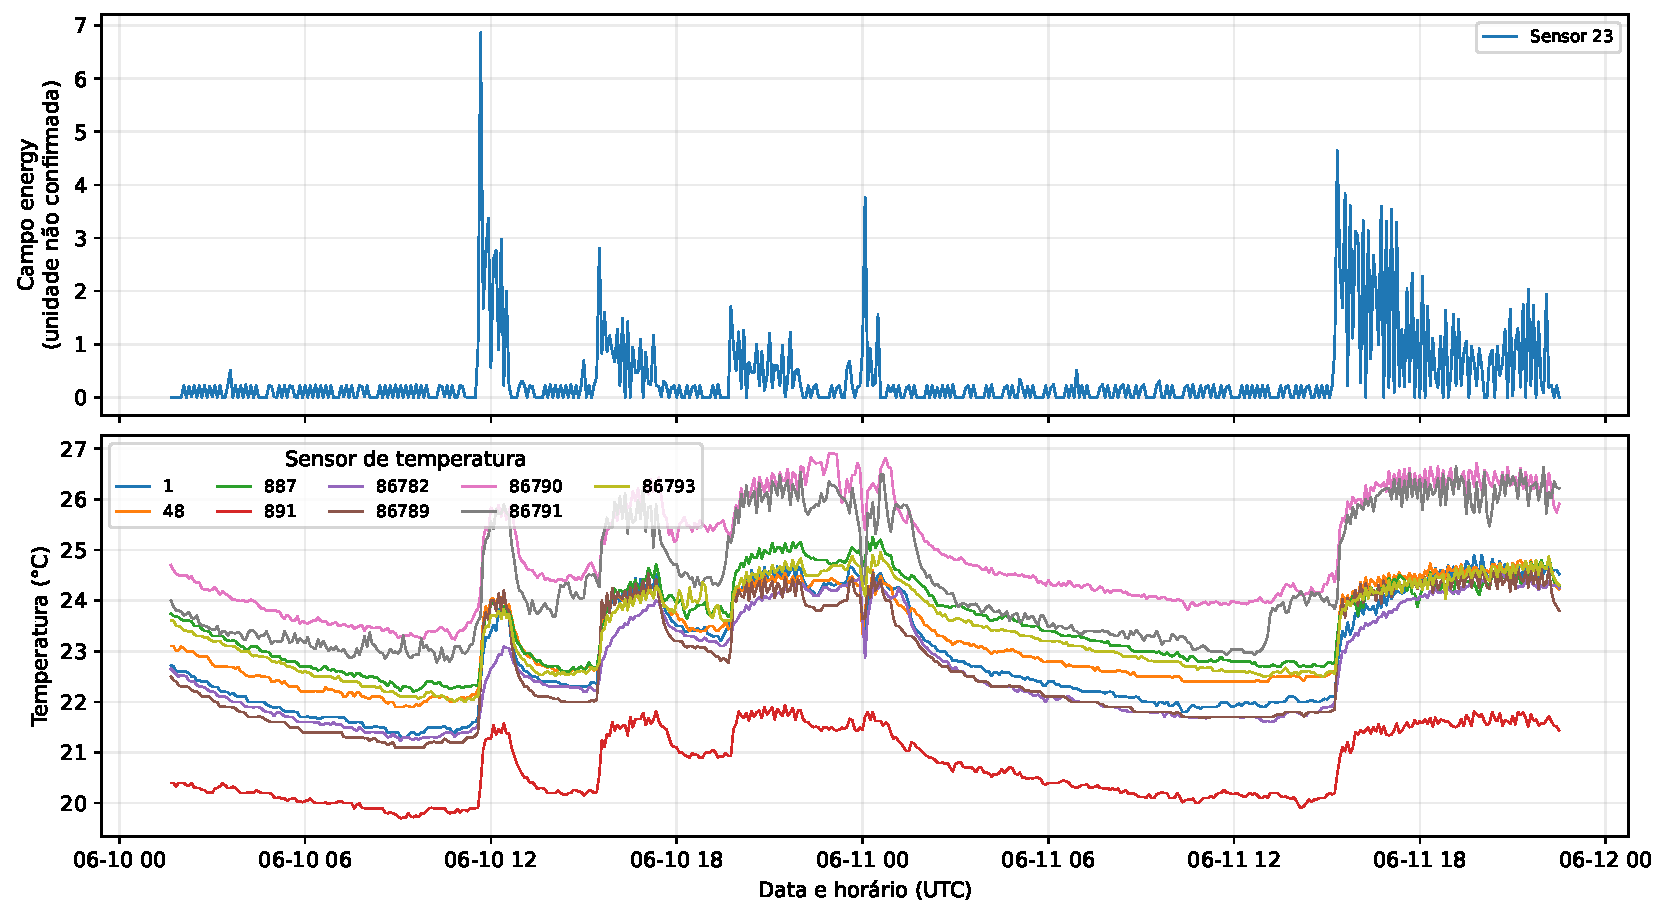
\includegraphics[width=\linewidth]{energia_temperatura_exploratoria.pdf}
    \fautor
\end{figure}

A série apresenta variações na escala registrada, mas sua sobreposição
às temperaturas não identifica, por si só, estados do ar-condicionado
ou efeitos causais. A curta disponibilidade e a unidade pendente de
confirmação limitaram o uso desses dados à auditoria e à visualização,
sem incluí-los como entradas dos modelos ou calcular consumo energético.

\subsection{Síntese e alcance dos resultados}
\label{subsec:sintese_resultados}

No conjunto estudado, foi possível reconstruir as médias de
temperatura dos nove sensores com MAE médio entre alvos próximo
de 0,25~°C usando métodos supervisionados. A adequação desse erro
a uma aplicação específica dependeria de requisitos que não foram
definidos neste experimento. A regressão linear e a Random Forest
apresentaram desempenho agregado próximo, com vantagens distintas
conforme a métrica e o alvo. A análise de quantidade mostrou que
mais entradas não asseguraram menor erro no período de teste.

A umidade acrescentou um ganho médio pequeno, com efeitos distintos
por alvo, enquanto os registros de energia tiveram disponibilidade
insuficiente para uma avaliação no período completo.
A evidência se restringe à reconstrução de janelas completas em
um ambiente e uma divisão temporal. Não foi avaliada a operação
sob indisponibilidade simultânea das entradas, nem a estabilidade
em outras estações, ambientes ou configurações físicas. Além disso,
a referência é a medição do sensor físico: concordância com esse
registro não demonstra exatidão em relação a um instrumento calibrado,
nem valida índices de conforto térmico ou um campo térmico contínuo.
